\PassOptionsToPackage{unicode=true}{hyperref} % options for packages loaded elsewhere
\PassOptionsToPackage{hyphens}{url}
%
\documentclass[brazil,12pt]{report}
\usepackage{lmodern}
\usepackage{amssymb,amsmath}
\usepackage{ifxetex,ifluatex}
\usepackage{fixltx2e} % provides \textsubscript
\ifnum 0\ifxetex 1\fi\ifluatex 1\fi=0 % if pdftex
  \usepackage[T1]{fontenc}
  \usepackage[utf8]{inputenc}
  \usepackage{textcomp} % provides euro and other symbols
\else % if luatex or xelatex
  \usepackage{unicode-math}
  \defaultfontfeatures{Ligatures=TeX,Scale=MatchLowercase}
\fi
% use upquote if available, for straight quotes in verbatim environments
\IfFileExists{upquote.sty}{\usepackage{upquote}}{}
% use microtype if available
\IfFileExists{microtype.sty}{%
\usepackage[]{microtype}
\UseMicrotypeSet[protrusion]{basicmath} % disable protrusion for tt fonts
}{}
\IfFileExists{parskip.sty}{%
\usepackage{parskip}
}{% else
\setlength{\parindent}{0pt}
\setlength{\parskip}{6pt plus 2pt minus 1pt}
}
\usepackage{hyperref}
\hypersetup{
            pdftitle={Probabilidade e Estatística com R},
            pdfauthor={Fernando Náufel},
            pdfborder={0 0 0},
            breaklinks=true}
\urlstyle{same}  % don't use monospace font for urls
\usepackage{color}
\usepackage{fancyvrb}
\newcommand{\VerbBar}{|}
\newcommand{\VERB}{\Verb[commandchars=\\\{\}]}
\DefineVerbatimEnvironment{Highlighting}{Verbatim}{commandchars=\\\{\}}
% Add ',fontsize=\small' for more characters per line
\usepackage{framed}
\definecolor{shadecolor}{RGB}{248,248,248}
\newenvironment{Shaded}{\begin{snugshade}}{\end{snugshade}}
\newcommand{\AlertTok}[1]{\textcolor[rgb]{0.94,0.16,0.16}{#1}}
\newcommand{\AnnotationTok}[1]{\textcolor[rgb]{0.56,0.35,0.01}{\textbf{\textit{#1}}}}
\newcommand{\AttributeTok}[1]{\textcolor[rgb]{0.77,0.63,0.00}{#1}}
\newcommand{\BaseNTok}[1]{\textcolor[rgb]{0.00,0.00,0.81}{#1}}
\newcommand{\BuiltInTok}[1]{#1}
\newcommand{\CharTok}[1]{\textcolor[rgb]{0.31,0.60,0.02}{#1}}
\newcommand{\CommentTok}[1]{\textcolor[rgb]{0.56,0.35,0.01}{\textit{#1}}}
\newcommand{\CommentVarTok}[1]{\textcolor[rgb]{0.56,0.35,0.01}{\textbf{\textit{#1}}}}
\newcommand{\ConstantTok}[1]{\textcolor[rgb]{0.00,0.00,0.00}{#1}}
\newcommand{\ControlFlowTok}[1]{\textcolor[rgb]{0.13,0.29,0.53}{\textbf{#1}}}
\newcommand{\DataTypeTok}[1]{\textcolor[rgb]{0.13,0.29,0.53}{#1}}
\newcommand{\DecValTok}[1]{\textcolor[rgb]{0.00,0.00,0.81}{#1}}
\newcommand{\DocumentationTok}[1]{\textcolor[rgb]{0.56,0.35,0.01}{\textbf{\textit{#1}}}}
\newcommand{\ErrorTok}[1]{\textcolor[rgb]{0.64,0.00,0.00}{\textbf{#1}}}
\newcommand{\ExtensionTok}[1]{#1}
\newcommand{\FloatTok}[1]{\textcolor[rgb]{0.00,0.00,0.81}{#1}}
\newcommand{\FunctionTok}[1]{\textcolor[rgb]{0.00,0.00,0.00}{#1}}
\newcommand{\ImportTok}[1]{#1}
\newcommand{\InformationTok}[1]{\textcolor[rgb]{0.56,0.35,0.01}{\textbf{\textit{#1}}}}
\newcommand{\KeywordTok}[1]{\textcolor[rgb]{0.13,0.29,0.53}{\textbf{#1}}}
\newcommand{\NormalTok}[1]{#1}
\newcommand{\OperatorTok}[1]{\textcolor[rgb]{0.81,0.36,0.00}{\textbf{#1}}}
\newcommand{\OtherTok}[1]{\textcolor[rgb]{0.56,0.35,0.01}{#1}}
\newcommand{\PreprocessorTok}[1]{\textcolor[rgb]{0.56,0.35,0.01}{\textit{#1}}}
\newcommand{\RegionMarkerTok}[1]{#1}
\newcommand{\SpecialCharTok}[1]{\textcolor[rgb]{0.00,0.00,0.00}{#1}}
\newcommand{\SpecialStringTok}[1]{\textcolor[rgb]{0.31,0.60,0.02}{#1}}
\newcommand{\StringTok}[1]{\textcolor[rgb]{0.31,0.60,0.02}{#1}}
\newcommand{\VariableTok}[1]{\textcolor[rgb]{0.00,0.00,0.00}{#1}}
\newcommand{\VerbatimStringTok}[1]{\textcolor[rgb]{0.31,0.60,0.02}{#1}}
\newcommand{\WarningTok}[1]{\textcolor[rgb]{0.56,0.35,0.01}{\textbf{\textit{#1}}}}
\usepackage{longtable,booktabs}
% Fix footnotes in tables (requires footnote package)
\IfFileExists{footnote.sty}{\usepackage{footnote}\makesavenoteenv{longtable}}{}
\usepackage{graphicx,grffile}
\makeatletter
\def\maxwidth{\ifdim\Gin@nat@width>\linewidth\linewidth\else\Gin@nat@width\fi}
\def\maxheight{\ifdim\Gin@nat@height>\textheight\textheight\else\Gin@nat@height\fi}
\makeatother
% Scale images if necessary, so that they will not overflow the page
% margins by default, and it is still possible to overwrite the defaults
% using explicit options in \includegraphics[width, height, ...]{}
\setkeys{Gin}{width=\maxwidth,height=\maxheight,keepaspectratio}
% Make links footnotes instead of hotlinks:
\DeclareRobustCommand{\href}[2]{#2\footnote{\url{#1}}}
\setlength{\emergencystretch}{3em}  % prevent overfull lines
\providecommand{\tightlist}{%
  \setlength{\itemsep}{0pt}\setlength{\parskip}{0pt}}
\setcounter{secnumdepth}{5}

% set default figure placement to htbp
\makeatletter
\def\fps@figure{htbp}
\makeatother


\hypersetup{
  colorlinks,
  breaklinks
}

% Lexend font
\usepackage{fontspec}
\setmainfont{Lexend Medium}
\setsansfont{Roboto} 


% Para bibliografia em português
\usepackage{babelbib}

% Para títulos de capítulos e seções:
\usepackage[nobottomtitles*]{titlesec}

%%%%%%%%%%%%%%%
%
% Titulos de capítulos e seções

\titleformat{\chapter}[display]%
{\bfseries\Large}%
{\filleft\MakeUppercase{\chaptertitlename} \Huge\thechapter}%
{4ex}%
{\titlerule%
  \vspace{2ex}%
  \filright}%
[\vspace{2ex}%
\titlerule%
\vspace{10ex}]

\titleformat{\section}[block]%
{\bfseries\Large}%
{\thesection}{.5em}{\titlerule\\[.8ex]\bfseries}

\titleformat{\subsection}[block]%
{\bfseries}%
{\thesubsection}{.5em}{\titlerule\\[.8ex]\bfseries}


%%%%%%%%%%%%%%%
%
% Caixas

\usepackage{tcolorbox}

\tcbset{
  sharp corners,
  boxrule=0.3mm,
  colback=black!2!white
}

\newtcolorbox{rmdbox}{
  colframe=black!40!white,
}

\newtcolorbox{mycaution}{
  colframe=red!75!black,
  sidebyside,
  lower separated=false,
  lefthand width=1cm,
  sidebyside gap=4mm
}

\newenvironment{rmdcaution}
{
  \begin{mycaution}
    
\includegraphics{images/caution.png}
    \tcblower
  }
  {
  \end{mycaution}
}

\newtcolorbox{myimportant}{
  colframe=green!75!black,
  sidebyside,
  lower separated=false,
  lefthand width=1cm,
  sidebyside gap=4mm
}

\newenvironment{rmdimportant}
{
  \begin{myimportant}
    
\includegraphics{images/important.png}
    \tcblower
  }
  {
  \end{myimportant}
}

\newtcolorbox{mywarning}{
  colframe=yellow!80!black,
  sidebyside,
  lower separated=false,
  lefthand width=1cm,
  sidebyside gap=4mm
}

\newenvironment{rmdwarning}
{
  \begin{mywarning}
    
\includegraphics{images/warning.png}
    \tcblower
  }
  {
  \end{mywarning}
}

\newtcolorbox{mynote}{
  colframe=yellow!70!black,
  sidebyside,
  lower separated=false,
  lefthand width=1cm,
  sidebyside gap=4mm
}

\newenvironment{rmdnote}
{
  \begin{mynote}
    
\includegraphics{images/note.png}
    \tcblower
  }
  {
  \end{mynote}
}

\newtcolorbox{mytip}{
  colframe=blue!50!white,
  sidebyside,
  lower separated=false,
  lefthand width=1cm,
  sidebyside gap=4mm
}

\newenvironment{rmdtip}
{
  \begin{mytip}
    
\includegraphics{images/tip.png}
    \tcblower
  }
  {
  \end{mytip}
}
\usepackage{booktabs}
\usepackage{longtable}
\usepackage{array}
\usepackage{multirow}
\usepackage{wrapfig}
\usepackage{float}
\usepackage{colortbl}
\usepackage{pdflscape}
\usepackage{tabu}
\usepackage{threeparttable}
\usepackage{threeparttablex}
\usepackage[normalem]{ulem}
\usepackage{makecell}
\usepackage{xcolor}
\ifnum 0\ifxetex 1\fi\ifluatex 1\fi=0 % if pdftex
  \usepackage[shorthands=off,main=brazil]{babel}
\else
  % load polyglossia as late as possible as it *could* call bidi if RTL lang (e.g. Hebrew or Arabic)
  \usepackage{polyglossia}
  \setmainlanguage[]{brazil}
\fi
\usepackage[]{natbib}
\bibliographystyle{apalike}

\title{Probabilidade e Estatística com R}
\author{Fernando Náufel}
\date{29/10/2021}

\begin{document}
\maketitle

{
\setcounter{tocdepth}{1}
\tableofcontents
}
\hypertarget{apresentacao}{%
\chapter*{Apresentação}\label{apresentacao}}
\addcontentsline{toc}{chapter}{Apresentação}

\hypertarget{oque}{%
\chapter{O Que É Estatística?}\label{oque}}

\hypertarget{vuxeddeo-1}{%
\section{Vídeo 1}\label{vuxeddeo-1}}

\begin{center} \url{https://youtu.be/6Q_XSoLCIpc} \end{center}

\hypertarget{exercuxedcios}{%
\section{Exercícios}\label{exercuxedcios}}

\begin{enumerate}
\def\labelenumi{\arabic{enumi}.}
\item
  Você está interessado em estimar a altura de todos os homens da sua faculdade. Para isso, você decide medir as alturas de todos os homens da sua turma de Estatística.

  \begin{itemize}
  \tightlist
  \item
    Qual é a amostra?
  \item
    Qual é a população?
  \end{itemize}
\item
  Um instituto de pesquisa entrevista um grupo de \(1000\) pessoas, perguntando a cada uma se ela vai votar a favor do candidato \(A\) na próxima eleição. Dos entrevistados, \(600\) responderam que sim. A proporção \(0{,}6\) (ou \(60\%\)) é uma estatística ou um parâmetro?
\item
  Você vê alguma diferença entre as cinco situações abaixo? Quais das situações são equivalentes em termos da probabilidade de conseguir \(5\) cartas do mesmo naipe?

  \begin{enumerate}
  \def\labelenumii{\alph{enumii}.}
  \item
    Usando um baralho normal, você retira \(10\) cartas e registra as cartas retiradas.
  \item
    Usando um baralho normal, você repete a seguinte sequência de ações \(10\) vezes: retirar uma carta do baralho, registrar a carta retirada e repor a carta no baralho.
  \item
    Usando uma caixa contendo todas as cartas de \(1\) milhão de baralhos reunidos, você retira \(10\) cartas e registra as cartas retiradas.
  \item
    Usando uma caixa contendo todas as cartas de \(1\) milhão de baralhos reunidos, você repete a seguinte sequência de ações \(10\) vezes: retirar uma carta da caixa, registrar a carta retirada e repor a carta na caixa.
  \item
    Usando um baralho \emph{infinito}, você retira \(10\) cartas e registra as cartas retiradas.
  \item
    Usando um baralho \emph{infinito}, você repete a seguinte sequência de ações \(10\) vezes: retirar uma carta do baralho, registrar a carta retirada e repor a carta no baralho.
  \end{enumerate}
\item
  Qual a graça dos quadrinhos na Figura \ref{fig:xkcd-cor}, que também \href{https://youtu.be/6Q_XSoLCIpc?t=1385}{aparecem no vídeo}?

  \begin{figure}

   {\centering 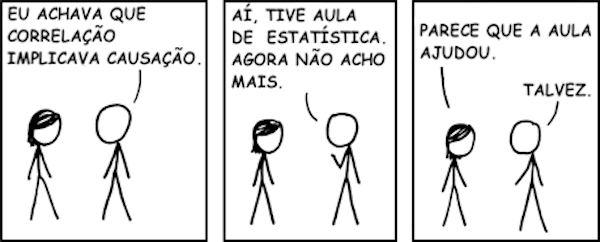
\includegraphics[width=0.9\linewidth]{images/correlation-pt-600} 

   }

   \caption{\url{http://xkcd.com/552/}}\label{fig:xkcd-cor}
   \end{figure}
\item
  Qual a graça dos quadrinhos na Figura \ref{fig:xkcd-blind}?

  \begin{figure}

   {\centering 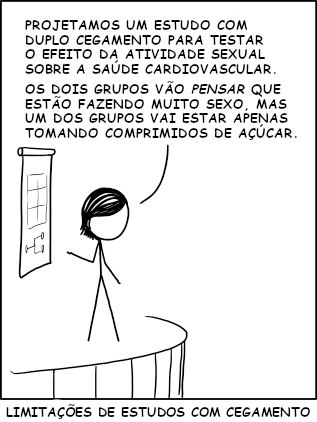
\includegraphics[width=0.5\linewidth]{images/double-blind} 

   }

   \caption{\url{http://xkcd.com/1462/}}\label{fig:xkcd-blind}
   \end{figure}
\item
  Veja este vídeo sobre o cavalo Hans:

  \begin{center} \url{https://youtu.be/G3VkCmdUfZE} \end{center}

  Qual a relação entre esta história e a necessidade de duplo cegamento?
\end{enumerate}





\hypertarget{vuxeddeo-2}{%
\section{Vídeo 2}\label{vuxeddeo-2}}

\begin{center} \url{https://youtu.be/492VASxlDRo} \end{center}

\hypertarget{exercuxedcios-1}{%
\section{Exercícios}\label{exercuxedcios-1}}

\begin{enumerate}
\def\labelenumi{\arabic{enumi}.}
\item
  Por que não faz sentido calcular a média dos CEPs de um grupo de pessoas?
\item
  Uma temperatura de \(-40\) graus Celsius é igual a uma temperatura de \(-40\) graus Fahrenheit?
\item
  Uma temperatura de zero graus Celsius é igual a uma temperatura de zero graus Fahrenheit?
\item
  Uma variação de temperatura de \(1\) grau Celsius é igual a uma variação de temperatura de \(1\) grau Fahrenheit?
\item
  Um saldo bancário de zero reais é igual a um saldo bancário de zero dólares?
\item
  Um produto de \(1\) milhão de reais custa o mesmo que um produto de \(1\) milhão de dólares?
\item
  Meses representados por números de \(1\) a \(12\) são dados de que nível?
\end{enumerate}

\hypertarget{rintro}{%
\chapter{Introdução a R}\label{rintro}}

\hypertarget{vuxeddeo-1-1}{%
\section{Vídeo 1}\label{vuxeddeo-1-1}}

\begin{center} \url{https://youtu.be/1kXQDNqm41c} \end{center}

\hypertarget{vuxeddeo-2-1}{%
\section{Vídeo 2}\label{vuxeddeo-2-1}}

\begin{center} \url{https://youtu.be/3GEc1oiKDrU} \end{center}

\hypertarget{exercuxedcios-2}{%
\section{Exercícios}\label{exercuxedcios-2}}

\begin{enumerate}
\def\labelenumi{\arabic{enumi}.}
\item
  Para criar sua conta no RStudio Cloud, acesse \url{https://rstudio.cloud/}.
\item
  Se você preferir instalar o R no seu computador, acesse

  \begin{itemize}
  \item
    \url{https://cran.r-project.org/} para baixar e instalar o R, e
  \item
    \url{https://rstudio.com/products/rstudio/download/} para baixar e instalar o RStudio, um IDE específico para R.
  \end{itemize}
\item
  Abra o RStudio Cloud ou o seu RStudio instalado localmente.
\item
  Crie um novo projeto. {Sempre trabalhe em projetos para ter seus arquivos organizados.}
\item
  Para instalar o \href{https://swirlstats.com/}{\texttt{swirl} (pacote do R para exercícios interativos)}, execute o seguinte comando no console do RStudio:

\begin{Shaded}
\begin{Highlighting}[]
\KeywordTok{install.packages}\NormalTok{(}\StringTok{"swirl"}\NormalTok{)}
\end{Highlighting}
\end{Shaded}
\item
  Para instalar os exercícios de introdução a R, execute os seguintes comandos no console do RStudio:

\begin{Shaded}
\begin{Highlighting}[]
\KeywordTok{library}\NormalTok{(swirl)}
\KeywordTok{install_course_github}\NormalTok{(}\StringTok{'fnaufel'}\NormalTok{, }\StringTok{'introR'}\NormalTok{)}
\end{Highlighting}
\end{Shaded}
\item
  Mude o idioma para português e execute o \texttt{swirl}.

\begin{Shaded}
\begin{Highlighting}[]
\KeywordTok{select_language}\NormalTok{(}\StringTok{'portuguese'}\NormalTok{, }\DataTypeTok{append_rprofile =} \OtherTok{TRUE}\NormalTok{)}
\KeywordTok{swirl}\NormalTok{()}
\end{Highlighting}
\end{Shaded}
\item
  Na primeira execução, você vai precisar se identificar (qualquer nome serve). Com essa identificação, o \texttt{swirl} vai registrar o seu progresso nas lições.
\item
  No \texttt{swirl}, as perguntas são mostradas no console. Você também deve responder no console.
\item
  Às vezes, um \emph{script} será aberto no editor de textos para que você complete um programa. Quando seu programa estiver pronto, salve o arquivo e digite \texttt{submit()} no console para o \texttt{swirl} processar o \emph{script}.
\item
  O \texttt{swirl} dá instruções claras no console. Na dúvida, digite \texttt{info()} no \emph{prompt} do R (\texttt{\textgreater{}}).
\item
  Se, em vez do \emph{prompt} do R, o console mostrar reticências (\texttt{...}), tecle \emph{Enter}.
\item
  Se nada funcionar, tecle \emph{ESC}.
\item
  Para sair do \texttt{swirl()}, digite \texttt{bye()} no \emph{prompt} do R.
\item
  Para voltar para os exercícios, digite

\begin{Shaded}
\begin{Highlighting}[]
\KeywordTok{library}\NormalTok{(swirl)}
\KeywordTok{swirl}\NormalTok{()}
\end{Highlighting}
\end{Shaded}
\end{enumerate}

\end{document}
